\documentclass[a4paper,12pt]{article}
\usepackage{geometry}
 \geometry{
 a4paper,
 total={210mm,297mm},
 left=20mm,
 right=20mm,
 bottom=20mm,
 top=20mm,
 }
\usepackage[english]{babel}
\usepackage[T1]{fontenc}
\usepackage{xcolor}
\usepackage[utf8]{inputenc}
\usepackage{lmodern}
\usepackage{microtype}
\usepackage{graphicx}
\usepackage{caption} 
\usepackage{titling}
\usepackage[colorlinks=true,linkcolor=black,urlcolor=blue]{hyperref}
\usepackage{indentfirst}
\usepackage{siunitx}
\usepackage{amsmath}
\usepackage{multicol}
\usepackage{enumitem}
\usepackage{listings}
\usepackage{matlab-prettifier}
\usepackage{pifont}

\title{Signals \& Systems II  Project\\[1ex]\large Processing motion signals from a PTZ camera}
\author{Curtil - Mafille - Maillard}

\date{January 7\textsuperscript{th}, 2024}

\begin{document}

\begin{titlepage}
    \centering
    \vspace{3cm}
    \Huge{\color{blue}\textbf{CT.2306 : Signal  \& Systems II }}\\
    \vspace{1cm}
    \Huge{\textbf{Report}}\\
    \vspace{0.5cm}
    \Large{Processing motion signals from a PTZ camera} \\
    \vspace{1cm}
    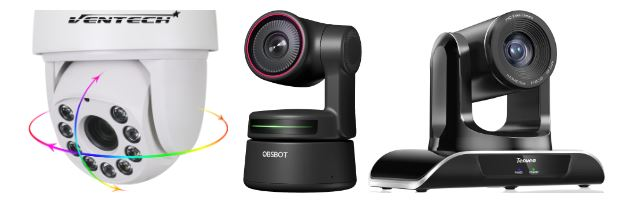
\includegraphics[scale=1]{Images/camera.jpg}\\
    \vspace{1.5cm}
    Philéas CURTIL, Thomas MAFILLE, Rémy MAILLARD \\
    \vspace{0.5cm}
    \vspace{1.5cm}
    \thedate \\
    \vspace{2cm}
    
\includegraphics[scale=0.7]{Images/Isep.jpg}\\
    \vspace{2cm}
    \small{\textit{Made with LaTeX}}

\end{titlepage}

\tableofcontents
\setlength{\parskip}{10pt}

\newpage

\section{Data visualization}

\begin{enumerate}[label={\color{blue}\arabic*)}]

    \item
    When we load \textit{data-proj.mat}, we can see that there are two vectors in the file :
    \begin{lstlisting}[style=Matlab-editor,language=Matlab]
    Name       Size

    omega      1x20001
    t          1x20001

    \end{lstlisting}

    \item
    Plot of the angular speed \(omega\) as a function of time.

    \begin{multicols}{2}

        \begin{flushleft}
            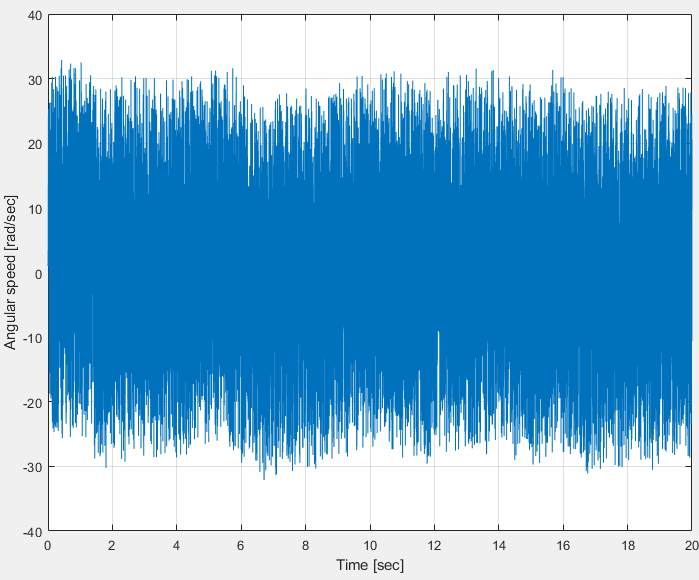
\includegraphics[scale=0.35]{Images/Figure 1.png}
            \captionof{figure}{Angular speed as a function of time}
            \label{Figure1}
        \end{flushleft}

    \columnbreak

    To obtain this graph :

    \begin{lstlisting}[style=Matlab-editor,language=Matlab, basicstyle=\small\ttfamily]
figure(1)
plot(t, omega)
grid on
hold on
xlabel('Time [sec]')
ylabel('Angular speed [rad/sec]')
        \end{lstlisting}

    \end{multicols}

    It is not possible to use the signal as it is now, mostly because there is too much information (too noisy) or the window is too large. This signal is continuous (analog). Electronic control devices requires digital signals.

\end{enumerate}

\newpage
\section{Analog filtering}

\begin{enumerate}[label={\color{blue}\arabic*)}]
    \setcounter{enumi}{2}
    \item The sampling period \(T_{e_1}\) can be calculated with :

        \begin{lstlisting}[style=Matlab-editor,language=Matlab, basicstyle=\small\ttfamily]
            Te1=t(2)-t(1)

            >>Te1 =

            1.0000e-03

        \end{lstlisting}

    \item
    Plot of the amplitude spectrum of \(omega(t)\), with the use of the workshop 5 :

    \begin{multicols}{2}

        \begin{flushleft}
            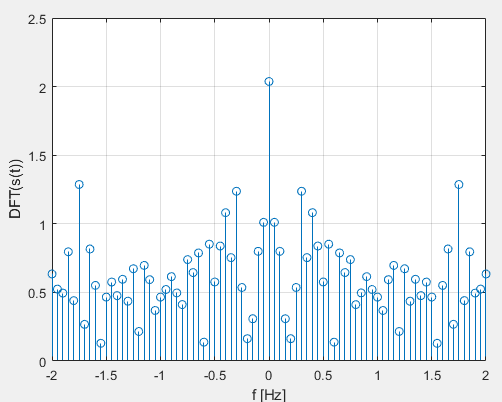
\includegraphics[scale=0.5]{Images/DFT.png}
            \captionof{figure}{DFT plot of \(omega(t)\)}
            \label{Figure2}
        \end{flushleft}

    \columnbreak

    To obtain this graph :

    \begin{lstlisting}[style=Matlab-editor,language=Matlab, basicstyle=\small\ttfamily]
% Plot of the DFT of omega(t)
Te2= 0.05; 
Fe1=1/Te1;
Tf=t(end);
N=Tf/Te1;

f1=-Fe1*(N/2-1)/N:Fe1/N:0;
f2=Fe1/N:Fe1/N:(N/2)*Fe1/N;
f = [f2,f1];
w= zeros(N,1);
for m=1:N
  for k=1:N
    w(m)=w(m)+omega(k)*exp(-1i*2*pi*m*k/N);
  
  end
end

figure(2)
stem(f,abs(w)/N)
grid on
xlim([-2 2])
xlabel('f [Hz]')
ylabel('Amplitude Spectrum of Angular Speed Signal')
        \end{lstlisting}

    \end{multicols}

    \item
    The frequencies contained inside the signal are ranging from -2 Hz to 2 Hz with a step of 0.05.

    \(F_{max} = 2 Hz\)
    \newpage

    \item
    The cutoff frequency is \(f_c = 2 Hz\). \\
    On Matlab :

    \begin{center}
        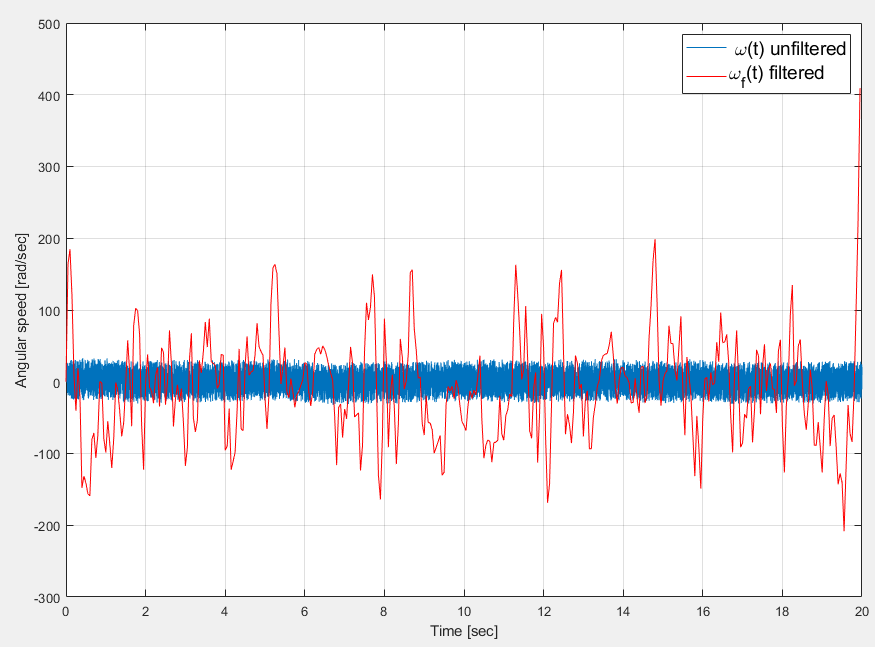
\includegraphics[scale=0.35]{Images/Omega_Filtered.png}
        \captionof{figure}{\(omega(t)\) filtered and unfiltered (\(omega_f(t)\))}
        \label{Figure3}
    \end{center}

    To obtain this graph :

    \begin{lstlisting}[style=Matlab-editor,language=Matlab, basicstyle=\small\ttfamily]
% filter design
t1=0:Te1:t(end)-Te1;
fc=0.2;
wc=2*pi*fc;

H1=tf(1,[1/(2*pi*fc)  1]);
wf=lsim(H1,omega,t);

% plot of filtered signal
figure(1);
plot(t,wf,'r')
hold off
grid on
legend(' omega(t) unfiltered','omega_{f}(t) filtered','Fontsize',14)
        \end{lstlisting}

 \newpage
    On Simulink :
    \begin{center}
        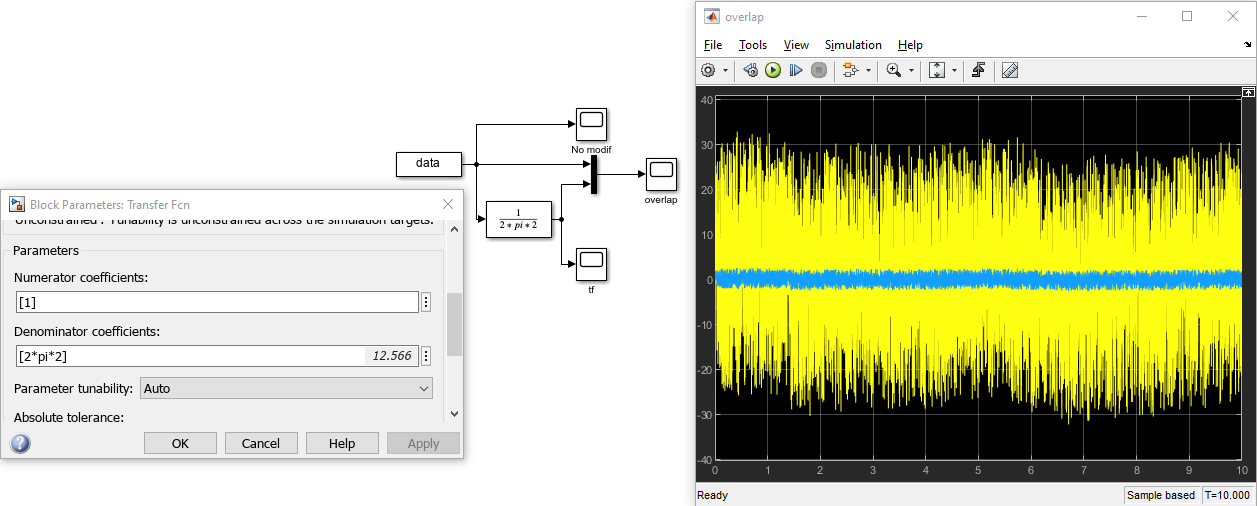
\includegraphics[scale=0.70]{Images/Simulink.png}
        \captionof{figure}{Simulink}
        \label{Figure4}
    \end{center}


    We need to add a part in the Matlab code as well :

    \begin{lstlisting}[style=Matlab-editor,language=Matlab, basicstyle=\small\ttfamily]
data = [t',omega'];
        \end{lstlisting}
        
    \item
    Plot of the amplitude spectrum of \(omega_f(t)\), with the use of the workshop 5 :

    \begin{center}
        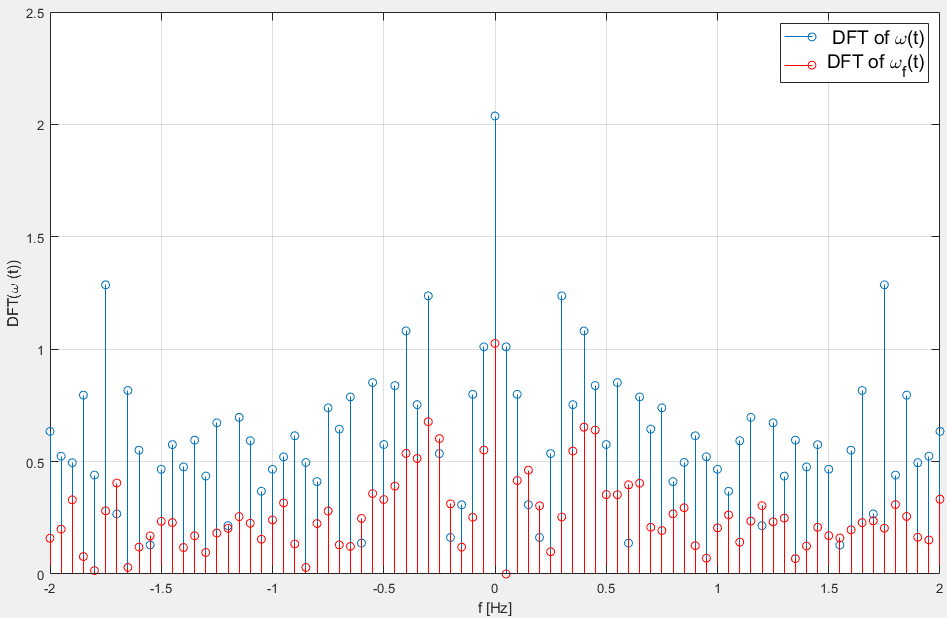
\includegraphics[scale=0.5]{Images/DFT_omega_f.png}
        \captionof{figure}{DFT plot of \(omega(t)\) and \(omega_f(t)\)}
        \label{Figure5}
    \end{center}

    \newpage
    To obtain this graph :

    \begin{lstlisting}[style=Matlab-editor,language=Matlab, basicstyle=\small\ttfamily]
wf1=zeros(N,1);
for m = 1 : N
    for k = 1 : N
        wf1(m) = wf1(m) + wf(k) * exp(-1i*2*pi*m*k/N);
    end
end

figure(3)
subplot(2,1,1);
stem(f,abs(w)/N), hold on
stem(f,abs(wf1)/N, 'r'), hold off
grid on
xlim([-100 100])
legend(' DFT of omega(t)','DFT of omega_{f}(t)','Fontsize',14)
title('DFT(w(t) and DFT(w_{f}(t) within [-100,100] Hz')

subplot(2,1,2);
stem(f,abs(w)/N), hold on
stem(f,abs(wf1)/N, 'r'), hold off
grid on
xlim([-2 2])
legend(' DFT of omega(t)','DFT of omega_{f}(t)','Fontsize',14)
title('DFT(w(t) and DFT(w_{f}(t) within [-2,2] Hz')
    \end{lstlisting}
        
\end{enumerate}

\newpage
\section{Sampling}

\begin{enumerate}[label={\color{blue}\arabic*)}]
    \setcounter{enumi}{7}

    \item
    To create a vector \(omega_e(t)\) which contains the values of the vector \(omega_f(t)\) with a period between the values of \(T_{e2}\) = 0.05 sec.
    \begin{lstlisting}[style=Matlab-editor,language=Matlab, basicstyle=\small\ttfamily]
temp1 = 1:round(Te2/Te1):length(t);
we=wf(temp1);
Te = t(temp1);
        \end{lstlisting}

    \item
    To get the size of \(omega_e(t)\), we use :
    \begin{lstlisting}[style=Matlab-editor,language=Matlab, basicstyle=\small\ttfamily]
>> size(we)

ans =

   401     1
        \end{lstlisting}
    

    \item
    The new vector \(t_e\) which corresponds to the vector \(omega_e(t)\) can be created using :
    \begin{lstlisting}[style=Matlab-editor,language=Matlab, basicstyle=\small\ttfamily]
temp1 = 1:round(Te2/Te1):length(t);
we=wf(temp1);
Te = t(temp1);
        \end{lstlisting}

    \item
    Plot of \(omega_f(t)\) and \(omega_e(t)\) :
    \begin{multicols}{2}
        \begin{flushleft}
            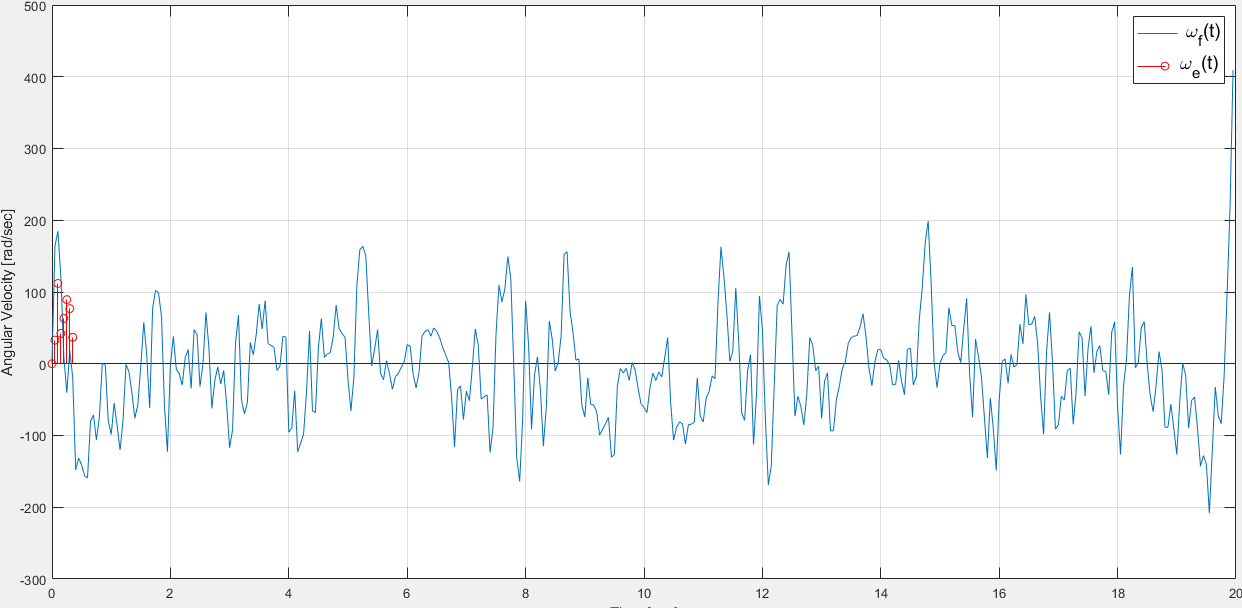
\includegraphics[width=0.95\linewidth]{Images/Wf_and_We.png}
            \captionof{figure}{Plot of \(omega_f(t)\) and \(omega_e(t)\)}
            \label{Figure7}
        \end{flushleft}

        \columnbreak

        \begin{lstlisting}[style=Matlab-editor,language=Matlab, basicstyle=\small\ttfamily]
figure(4)
plot(t,wf), hold on
xlabel('Time [sec]')
ylabel('Angular Velocity [rad/sec]')
grid on
stem(Te,we, 'r'), hold off
legend(' omega_{f}(t)','omega_{e}(t)','Fontsize',14)
        \end{lstlisting}
    \end{multicols}

    \newpage

    To plot the graph between 10 and 12, we add xlim([10 12]) to the Matlab code.
    \begin{multicols}{2}
        \begin{flushleft}
            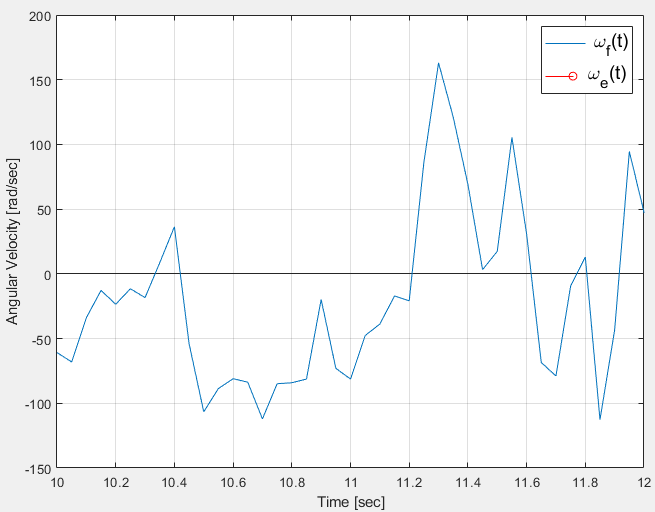
\includegraphics[width=0.75\linewidth]{Images/Wf_and_We_Zoomed.png}
            \captionof{figure}{Plot of \(omega_f(t)\) and \(omega_e(t)\), focused between 10 and 12}
            \label{Figure8}
        \end{flushleft}

        \columnbreak

        \begin{lstlisting}[style=Matlab-editor,language=Matlab, basicstyle=\small\ttfamily]
figure(4)
plot(t,wf), hold on
xlim([10 12])
xlabel('Time [sec]')
ylabel('Angular Velocity [rad/sec]')
grid on
stem(Te,we, 'r'), hold off
legend(' omega_{f}(t)','omega_{e}(t)','Fontsize',14)
        \end{lstlisting}
    \end{multicols}

    \item
    Plot of \(omega(t)\), \(omega_f(t)\) and \(omega_e(t)\) :
    \begin{multicols}{2}
        \begin{flushleft}
            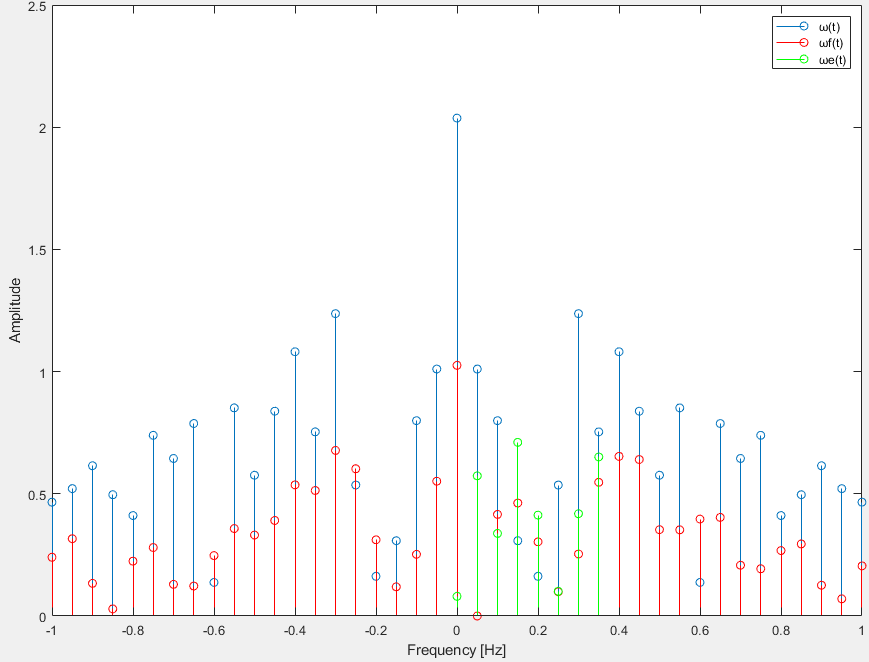
\includegraphics[width=1\linewidth]{Images/w_wf_weDFT.png}
            \captionof{figure}{Plot of \(omega_f(t)\) and \(omega_e(t)\)}
            \label{Figure9}
        \end{flushleft}

        \columnbreak

        \begin{lstlisting}[style=Matlab-editor,language=Matlab, basicstyle=\small\ttfamily]
Fe2=1/Te2;
Tf2=Te(end);
N2=Tf2/Te2;

f3=-Fe2*(N2/2-1)/N2:Fe2/N2:0;
f4=Fe2/N2:Fe2/N2:(N2/2)*Fe2/N2;
f_2=[f4,f3];

we_dft = zeros(N2,1);
for m = 1 : N2
    for k = 1 : N2
        we_dft(m) = we_dft(m) + we(k) * exp(-1i*2*pi*m*k/N2);
    end
end

figure(5)
stem(f,abs(w)/N), hold on
stem(f,abs(wf1)/N, 'r')
stem(f_2,abs(we_dft)/N2, 'g'), hold off
xlabel('Frequency [Hz]')
ylabel('DFT')
legend({'DFT of omega(t)', 'DFT of omega_f(t)', 'DFT of omega_e(t)'})
xlim([-2 2])
        \end{lstlisting}
    \end{multicols}

\end{enumerate}

\newpage
\section{Angular position and acceleration}

\begin{enumerate}[label={\color{blue}\arabic*)}]
    \setcounter{enumi}{12}

    \item
    To calculate the angular acceleration\(omega dot(t)\) and the position \(theta(t)\) :
     \begin{lstlisting}[style=Matlab-editor,language=Matlab, basicstyle=\small\ttfamily]
% angular acceleration
wd_start=(we(2)-we(1))/Te2;
wd_end=(we(end)-we(end-1))/Te2;
wd_mid=zeros(8,1);
for i=2:N2-1
    wd_mid(i)=(we(i+1)-we(i-1))/(2*Te2);
end

wd=[wd_start;wd_mid;wd_end];


% angular position
theta=zeros(N2,1);

for i=1:N2
    for k=1:i+2
        theta(i)=theta(i)+Te2*we(k);
    end
end
        \end{lstlisting}

    \item
    We can now plot the two graphs for \(theta(t)\) and \(omega'(t)\) :
    \begin{multicols}{2}
    \begin{flushleft}
            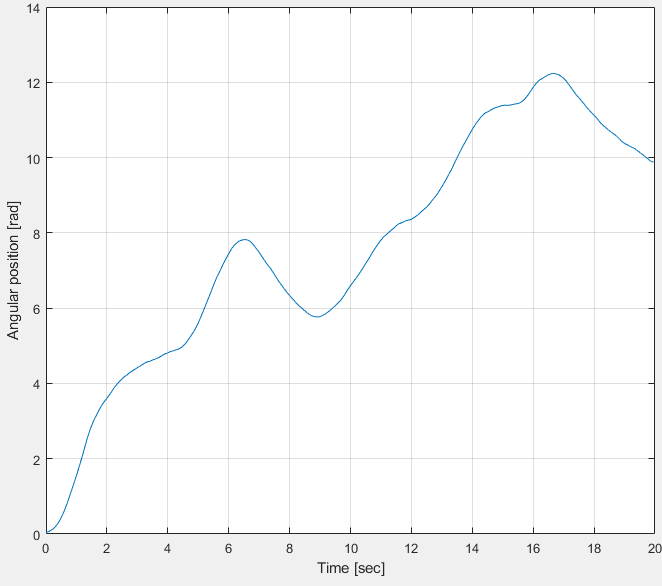
\includegraphics[width=1\linewidth]{Images/theta.png}
            \captionof{figure}{Plot of \(theta(t)\)}
            \label{Figure10}
        \end{flushleft}
    \columnbreak
    \begin{flushright}
            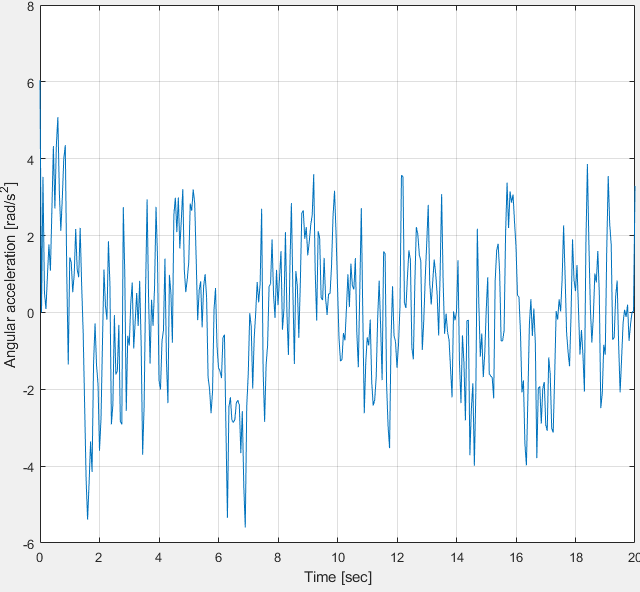
\includegraphics[width=1\linewidth]{Images/omega_dot.png}
            \captionof{figure}{Plot of \(omega'(t)\)}
            \label{Figure11}
        \end{flushright}
        
    \end{multicols}
    To get the plots :
    \begin{lstlisting}[style=Matlab-editor,language=Matlab, basicstyle=\small\ttfamily]
t_ang=0:Te2:Te(end)-Te2;

figure(6)
plot(t_ang, theta)
xlabel('Time [sec]')
ylabel('Angular position [rad]')
grid on

figure(7)
plot(Te,wd)
xlabel('Time [sec]')
ylabel('Angular acceleration [rad/s^2]')
grid on
        \end{lstlisting}
    

    \item
    The plot of the DFt of \(theta(t)\) and \(omega'(t)\) :
    \begin{multicols}{2}
    \begin{flushleft}
            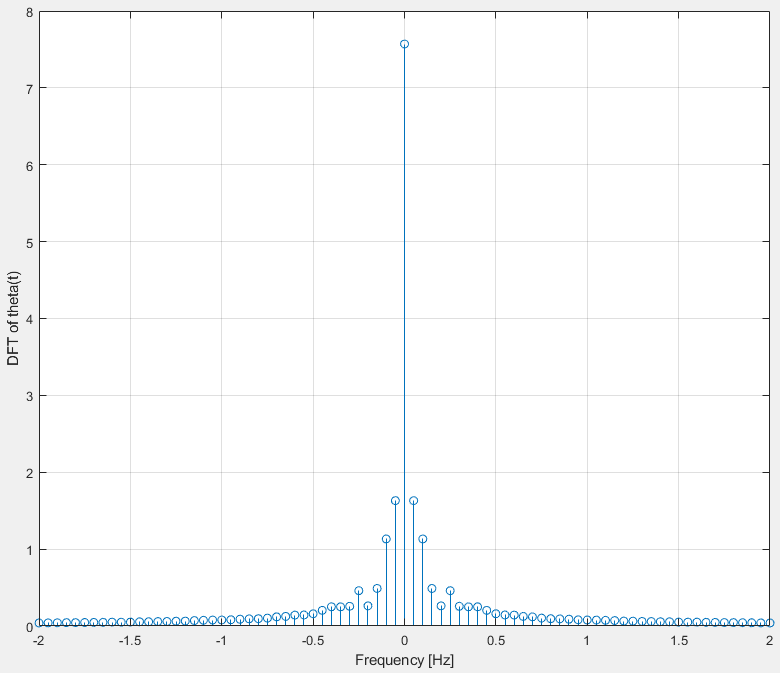
\includegraphics[width=1\linewidth]{Images/DFT_theta.png}
            \captionof{figure}{Plot of DFT(\(theta(t)\))}
            \label{Figure10}
        \end{flushleft}
    \columnbreak
    \begin{flushright}
            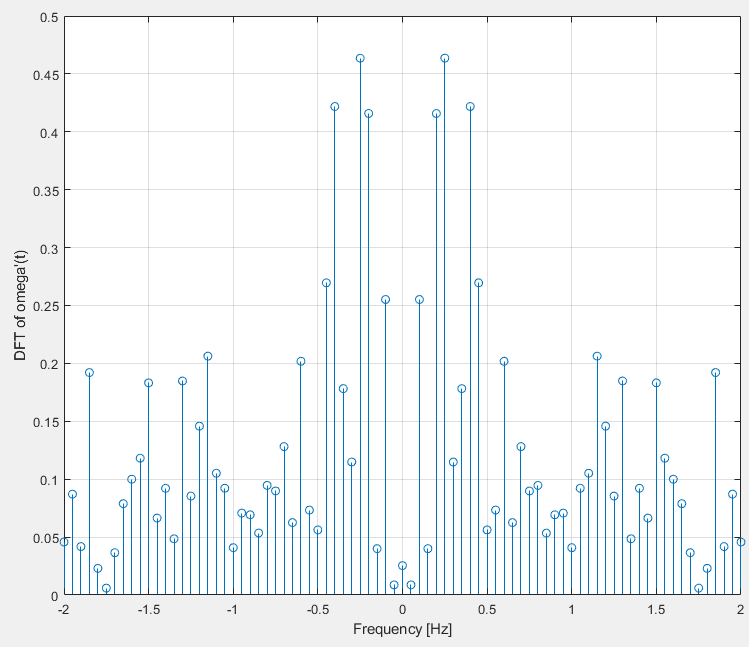
\includegraphics[width=1\linewidth]{Images/DFT_omega_dot.png}
            \captionof{figure}{Plot of DFT(\(omega'(t)\))}
            \label{Figure11}
        \end{flushright}
        
    \end{multicols}
    To get the plots and calculate the DFT of \(omega'(t)\) and \(theta(t)\) :
    \begin{lstlisting}[style=Matlab-editor,language=Matlab, basicstyle=\small\ttfamily]
wd_dft=zeros(N2,1);
for m=1:N2
    for k=1:N2
        wd_dft(m)=wd_dft(m)+wd(k)*exp(-1i*2*pi*m*k/N2);
    end
end

theta_dft = zeros(N2,1);
for m=1:N2
    for k=1:N2
        theta_dft(m)=theta_dft(m)+theta(k)*exp(-1i*2*pi*m*k/N2);
    end
end

figure(8)
stem(f_2,abs(theta_dft)/N2)
xlim([-2 2])
grid on
xlabel('Frequency [Hz]')
ylabel('DFT of theta(t)')

figure(9)
stem(f_2,abs(wd_dft)/N2)
xlim([-2 2])
grid on
xlabel('Frequency [Hz]')
ylabel("DFT of omega'(t)")
        \end{lstlisting}

\end{enumerate}

\newpage
\section{Digital filtering}

\begin{enumerate}[label={\color{blue}\arabic*)}]
    \setcounter{enumi}{15}

    \item
    A

    \item
    A

    \item
    A

\end{enumerate}

\end{document}